When exposed to naturalistic stimuli (e.g. movie watching or simulated driving), subjects' experience is closer to their every-day life than with classical
psychological experiments.
% 
This makes naturalistic paradigms an attractive class of
stimulation protocols for brain imaging.
%
However, such stimulations are difficult to quantify, therefore the statistical analysis of the data using supervised regression-based approaches is challenging.
This has motivated the use of unsupervised learning methods that do not make
assumptions about what triggers brain activations in the stimuli.

In this chapter, we first present \emph{independent component analysis} (ICA), a widely used
unsupervised method for neuro-imaging studies routinely applied on individual
subject electroencephalography (EEG)~\cite{makeig1996independent},
magnetoencephalography (MEG)~\cite{vigario1998independent} or functional MRI
(fMRI)~\cite{mckeown1998independent} data, then we review \emph{multiview} unsupervised 
techniques that leverage the availability of data from multiple subjects
performing the same experiments. 

\section{Independent component analysis}
\label{sec:ica}
Independent component analysis (ICA) models a set of signals as the product of a \emph{mixing matrix} and a
\emph{component} matrix containing independent components. As will be seen in this
section, the required assumptions on the independent components to guarantee
identifiability are rather weak making ICA a method of choice to analyze the
data of subjects exposed to a stimuli that is difficult to quantify.

ICA is applied in fMRI data to analyze resting state
data~\cite{beckmann2005investigations} or when subjects are
exposed to natural~\cite{malinen2007towards}~\cite{bartels2005brain} or complex stimuli~\cite{calhoun2002different}. 
In M/EEG processing, it is widely used to isolate acquisitions artifacts from neural signal~\cite{jung1998extended}, and to identify brain components of interest~\cite{vigario2000independent, delorme2012independent}.

In neuroscience, the number of components $k$ is typically much lower than the number
of available observations $v$. We are therefore in an overcomplete setting.
However in ICA, it is assumed the number of observations is equal to the number
of sources. Therefore, a
typical pre-processing step is to reduce the dimension. We therefore first
present principal component analysis which is the standard method to perform
dimension reduction in this context.

\subsection{Principal component analysis (PCA)}
Let us assume our data are given by a random vector $\xb \in \RR^{v}$. The data
are centered ($\EE[\xb] = 0$). Principal component analysis (PCA) gives an orthonormal familly of $p$ vectors $R \in \RR^{v \times p}$ such that projecting our data onto this family
using $R R^{\top} \xb$ does not yield a large reconstruction error in Frobenius
norm.
The corresponding optimization problem is given by:
\begin{align}
  &\argmin_{R} \|\xb - R R^{\top} \xb \|^2 \\
  &=\argmin_{R} \trace(  \xb^{\top}(I - R R^{\top}) (I - R R^{\top}) \xb\|^2 \\
  &= \argmin_{R} \|\xb \|^2 - \|R^{\top} \xb \|^2 \\
  &= \argmax_{R} \|R^{\top} \xb \|^2 \\
  &= \argmax_{R} \trace(R^{\top} \VV[\xb] R)
\end{align}
Therefore the matrix $R$ is just given by the first $p$ eigenvectors of
$\VV[\xb]$. In practice we observe a matrix of data $X \in \RR^{v, n}$ and
would compute an empirical estimate of the covariance by $\frac1{n}X X^{\top}$.
%
However, such an estimate is not practical in high dimensions: $v$ is very
large and therefore $XX^{\top}$ is a prohibitively large matrix.

Therefore, we rely instead of the singular value decomposition of $X$:
\begin{align}
X= U D V
\end{align}
  where $U \in \RR^{v \times t}$ is an orthogonal matrix ($U^{\top} U
= I_t$) of
\emph{left-singular vectors}, $D \in \RR^{t}$ is a positive diagonal matrix of
singular values and $V \in \RR^{t \times t}$ is an orthogonal matrix of
\emph{right-singular vectors}.
%
Every matrix has a singular value decomposition and this
decomposition is unique up to reordering of the singular vectors (and
corresponding permutations of the left/right singular vectors) and sign-flips of
the left and right singular vectors.

Let $X = UDV$ be a singular value decomposition of $X$, we have $XX^{\top}= U
D^2 U^{\top}$ and therefore the left-singular vectors $U_p$ corresponding to the
largest $p$ singular values of $X$ yield  the $p$ largest eigenvectors of
$XX^{\top}$.
Therefore $R = U_p$.

Sometimes the PCA includes whitening $R = U_p D_p^{-1}$ where $D_p$ contains the
 $p$ largest singular values of $X$ so that projected data are
uncorrelated (but $R$ is no longer orthonormal). In this paper what we call PCA
does not include whitening of the signals.

After the data are reduced such that the number of observations are identical to
the number of components, we can perform independent component analysis (ICA).
ICA can exploit a number of different properties of the signal. Most of our
algorithms use non-gaussianity of the data to extract relevant components so we
focus next on non-Gaussian ICA.

\subsection{Non Gaussian ICA}
ICA sees the data $\xb \in \RR^p$ as a linear mixtures of components $\sbb \in \RR^p$.
Data are therefore modeled as:
\begin{align}
  \xb = A \sbb
\end{align}
where $A$ is the unmixing matrix and $\sbb$ have a non-Gausian distribution.
Without loss of generality, the data $\xb$ are assumed centered ($\EE[\xb] = 0$).
This section relies heavily on the ICA review~\cite{hyvarinen2000independent}
and on~\cite{cardoso1997infomax}.

\subsubsection{Identifiability}
It is easily seen that if $\sbb$ is non-Gaussian, so is $P \sbb$ where  $P$ is a
sign and permutation matrix.
Therefore if $\xb = A \sbb$, take $A' = AP^{\top}$ and $\sbb'=P\sbb$ and we have
$\xb = A' \sbb'$.
In other words, there exist a permutation and scaling indeterminacy.

Therefore, we can assume without loss of generality that $\sbb$ has unit variance ($\VV[\sbb] = I$).
If we whiten the data by applying a matrix $H$ such that $\VV[H \xb] = I_p$ we have $H \xb = \tilde{A} \sbb$ where $\tilde{A} = HA$. $\VV[H \xb] = 1$ implies $\tilde{A}^{\top} \tilde{A} = I$ so without loss of generality we can assume that $\xb$ has unit variance and that $A$ is orthogonal. 

We now show that the previously described scale and permutation
indeterminacies are the only one.
Let us assume that there exists two mixing matrices $A_1$ and $A_2$ such that
$\xb = A_1 \sbb_1$ and $\xb = A_2 \sbb_2$ with $A_1$ and $A_2$ orthogonal. Then $\sbb_1 = O \sbb_2$ where $O = A_1^{\top} A_2 \sbb_2$.
The following theorem in~\cite{comon1994independent}
shows that $O$ can only be a scale and permutation matrix.
\begin{theorem}
  Let $\sbb_2$  be a  vector  with  independent 
  components, of   which  at  most  one  is  Gaussian,  and whose  densities
  are  not  reduced  to  a  point-like  mass. Let $O$ be an orthogonal matrix
  and $\sbb$ such that $\sbb = O \sbb_2$.
  Then, $\sbb$ has independent component if and only if $O$ is a scale and
  permutation matrix.
\end{theorem}

As a result, if we assume that at most one source is Gaussian, ICA is identifiable up to a scale and permutation indeterminacy.

\subsubsection{Infomax: Maximum likelihood estimation}
Infomax is introduced in~\cite{bell1995information} in the context of source
separation as maximizing the entropy of $g(W \xb) = g_i(\wb_i \xb)$ where  $g_i$
is differentiable, strictly increasing function with value in $]0, 1[$. As shown
in~\cite{cois1997infomax}, this is equivalent to
maximum likelihood where component $i$ is assumed to have $g_i$ as its
cumulative distribution function.

Assume for simplicity that the sources have the same density $\delta$, denoting $f(x) =
-\log(\delta(x))$ and $f(\xb) = \sum_{i=1}^m f(x_i)$ for $\xb \in
\RR^m$ the negative log-likelihood is given by:
\begin{align}
  \loss &= -l(\xb, \theta) = - \log(p(\xb)) \\
        &= -\log(|W|) - \log(\delta(W \xb)) \\
  &= -\log(|W|) + f(W \xb)
\end{align}
where we used the change of variable $\sbb = W \xb$.

\subsubsection{Optimizing the maximum likelihood: relative gradient, Hessian and approximations}
\label{sec:opt:likelihood:relativegradient}
The matrix $W$ needs to be invertible. In practice, if the constraint is not
enforced, we could see numerical instabilities appear.
A simple rule that preserve the inversibility of $W$ is to use updates of the
form:
\begin{align}
  W \leftarrow (I + \alpha D)W \label{eq:mult:update}
\end{align}
where $\alpha$ is a small step-size and $D$ is a direction to be found.
Following the same reasonning as in section~\ref{sec:gd}, we assume a small step-size
and write at first order:
\begin{align}
  \argmin_{D, \|D\|=1} \loss((I + \alpha D)W) &= \argmin_{D, \|D\|=1} \loss(W) + \langle \partialfrac{W}{f(W)} | \alpha D W \rangle \\
                                              &= \argmin_{D, \|D\|=1} \loss(W) + \langle \partialfrac{W}{f(W)} W^{\top} | \alpha D \rangle \\
                                              &= -\frac{\partialfrac{W}{f(W)} W^{\top}}{\|\partialfrac{W}{f(W)} W^{\top} \|}
\end{align}
The updates are therefore given by  $W \leftarrow (I - \alpha G)W$ where $G = \partialfrac{W}{f(W)}
  W^{\top}$ is called the \emph{relative
  gradient}~\cite{cardoso1996equivariant}.
Second order extensions of the method are obtained by following the steps in
section~\ref{sec:qn}. The corresponding Hessian is called the \emph{relative
  Hessian}.
As a side note, the relative gradient coincides with the natural
gradient~\cite{amari1999natural} that exploits the property of the statistical model.


Let us follow~\cite{ablin2018faster} and use a quasi-Newton algorithm to minimize the likelihood.
The relative gradient and Hessian of $\loss$ is given by:
\begin{align}
  G = f'(\yb) \yb^{\top} - I_p
\end{align}
where $\yb = W \xb$ and $f'(\yb) = \partialfrac{f(\yb)}{\yb}$
and
\begin{align}
  H_{abcd} =  \delta_{ad}\delta_{bc} + \delta_{ac} f''(y_a)y_by_d
\end{align}

Following~\cite{ablin2018faster}, we can approximate the Hessian by
\begin{align}
  \tilde{H}_{abcd} = \delta_{ad} \delta_{bc} + \delta_{ac} \delta_{bd} \Gamma_{ab}
\end{align}
where $\Gamma_{ab} = f''(y_a) y_b^2$.
The approximation is exact when the true unmixing matrix is found since $\EE[s_b s_d] =  s_b^2\delta_{bd}$.

The updates are then given by:
\begin{align}
  W \leftarrow (I - \alpha \tilde{H}^{-1} G) W
\end{align}

Note the abuse of notation here. In the update formula, we actually mean
$\EE[\tilde{H}]$ and $\EE[G]$,
instead of $\tilde{H}$ and $G$.
In practice, these expectations are replaced by empirical expectations. We often do such abuse in the rest of the thesis when it is clear from the context whether we mean random variables or their (empirical) expectation. 

Note that the term $\tilde{H}^{-1} G$ is particularly easy to compute. Indeed we
have:
\begin{align}
[\tilde{H}^{-1} G]_{ab} = \frac{\Gamma_{ba} G_{ab} - G_{ba}}{\Gamma_{ba}
  \Gamma_{ab} - 1}
\end{align}

\subsubsection{Robustness to density mismatch}
In practice, we observe that sometimes, the quasi-Newton algorithm described in
the previous section fails to recover the true mixing matrix. This happens when the
sources used in the model are too far from the true sources in the data. In this section, we explain
why this happens and derive stability conditions. This follows the work done in~\cite{cardoso1998blind}.

When the density of the sources correspond to the one used in the model. We
recover the correct unmixing matrices via the maximum likelihood estimate in the
limit of large samples. This comes from the consistency of maximum likelihood
estimators.
When this is not the case, a mismatch appears which can be quantified. Let us
denote $\xb^*$ the true data. As highlighted in~\eqref{kl-likelihood} the expected
negative log-likelihood coincides, up to a constant, with the KL divergence between the true
distribution of the data and the distribution of the data as hypothesized in the
model:
\begin{align}
  &-l(\theta) \\
  &=  D_{KL}(p(\xb^*), p(W^{-1} \sbb)) \\
             &=  D_{KL}(p(W\xb^*), p(\sbb)) \\
             &=  D_{KL}(p(W \xb^*), \prod_i p_i(\wb_i\xb^*)) + D_{KL}(\prod_i p_i(\wb_i\xb^*), p(\sbb)) \\
             &=  D_{KL}(p(W \xb^*), \prod_i p_i(\wb_i\xb^*)) + D_{KL}(\prod_i p_i(\wb_i\xb^*), \prod_i p_i(s_i)) \\
\end{align}
where the first equality comes from the invariance of the KL divergence and we
denote $\prod_i p_i(x_i)$ the product of the marginal densities of $\xb$.

The first term in the last equality is the mutual information. It quantifies the
independence of unmixed data $W \xb$. The second term quantifies the mismatch
between the assumed distribution of the sources and the marginals of unmixed data.
Therefore if the assumed sources are too far from the true sources, the
recovered unmixing matrices may be far from the true ones.


Looking at the relative gradient $G$, we see that if sources are truly
independent, the true unmixing matrix will be a stationary point of the loss up
to a scaling: $G(\Lambda A^{-1})=0$ where $\Lambda=\diag(\lambda_1 \dots \lambda_p)$.
However, in order for the quasi-Newton to reach this point, it must be a local
minima (the Hessian must be definite positive). 

Let us therefore consider the Hessian $H$ at point $W = \Lambda A^{-1}$ where
$\Lambda$ is chosen such that $G = 0$. The unmixed data $\yb = W \xb$ are independent and
therefore, we have $\tilde{H} = H$.
For any matrix $M$:
\begin{align}(\tilde{H} M)_{ab} = M_{ba} + M_{ab} f''(y_a)y_b^2
\end{align}.
So $\tilde{H}$ is block diagonal with blocks of size either 1 or 2.
The blocks of size 1 are given by :
\begin{align}
  1 + f''(y_a) y_a^2
  s_a^2
\end{align}
and the blocks of size
two are given by the matrix
\begin{align}
                              \begin{bmatrix} f''(y_a) y_b^2
  & 1 \\ 1 &
  f''(y_b)y_a^2 \end{bmatrix}
\end{align}
Therefore the conditions for stability are given by:
\begin{align}
  \forall a, b, a \neq b, \enspace \left(f''(y_a) y_a^2 \right) \left(f''(y_b)  y_b^2 \right) > 1
\end{align}

When the conditions are satisfied, the quasi-Newton algorithms will recover the
true unmixing matrices if initialized close to a solution. In practice, this
method recovers the correct unmixing matrices in a wide variety of cases.

\subsection{A variation : non-stationary ICA and joint diagonalization}
Up to now we have assumed that samples were independent an identically distributed. In non-stationary ICA, samples are no longer identically distributed as the distribution can vary over time.
This section follows the work in~\cite{pham2001blind}.
The sources are assumed to be Gaussian with a variance that varies between
samples but is assumed to be piece-wise constant $\Sigma_t = \Sigma_k$ for $t \in
T_k$ where $(T_k)_k$ is a partition of $[1, 2, \dots, n]$ and $\Sigma_k$ is a
positive diagonal matrix.

The (empirical) likelihood is given by:
\begin{align}  
  \loss &= -\log(|W|)  + \frac1{n} \sum_k \big( \frac12 \sum_{i \in T_k}\|\Sigma_k^{-\frac12} W \xb^k_i \|^2 + \frac12 \log(|\Sigma_k|) \big)
\end{align}
Denoting $C_k = \sum_{i \in T_k} \xb_i^k (\xb_i^k)^{\top}$ we have 

\begin{align}  
  \loss &= -\log(|W|)  + \frac1{n} \sum_k \big( \frac1{2} \trace(\Sigma_k^{-1} W C_k W^{\top}) + \frac12 \log(|\Sigma_k|) \big)
\end{align}
Minimizing $\loss$ with respect to $\sigma_k^2$ yields $\Sigma_k = \diag(W C_k
W^{\top})$ and therefore up to a constant:
\begin{align}  
  \loss &= -\log(|W|)  + \frac1{n} \sum_k \big(\frac12 \log(|\diag(W C_k W^{\top})|) \big)
\end{align}
which can be rewritten:
\begin{align}  
  \loss &=\frac1{2n} \sum_k \big(\frac{\log(|\diag(W C_k W^{\top})|)}{\log(W C_k W^{\top})} \big)
\end{align}

$\loss$ is a joint diagonalization criterion. The optimal $W$ can be found via a
quasi-Newton method very similar to the one we used for non-Gaussian
ICA~\cite{ablin2018beyond} however, performing ICA via joint diagonalization is
in principle much faster than using non-Gaussian ICA.

\section{Analysis of MultiView data}
In this section, we present multiview unsupervised techniques suited to
analyze the data of multiple subjects exposed to the same complex stimuli. Such
techniques assume some similarity between the data of different subjects. This
assumption can be justified by the findings of \cite{hasson2004intersubject} showing that brains exposed to the same natural stimuli exhibit synchronous activity.
The task of finding common patterns or responses that are shared between
subjects is called \emph{shared response modeling}.

In the general linear model presented in
section~\ref{sec:glm}, the shared response is assumed to be known. Therefore,
multiple subjects can be studied separately assuming the data of different
subjects are independent given the shared response.
In the unsupervised setting it may not be so straightforward to deal with
multiple subject and therefore many different
methods for data-driven multivariate analysis of neuroimaging group studies
have been proposed.
We summarize the characteristics of some of the most commonly used ones.


\subsection{Multiset canonical correlation analysis}
\label{sec:mcca}
Canonical correlation analysis is initially designed to find a linear
combination that maximizes the correlation between two datasets.
The extension to more than two datasets is ambiguous, and many
different generalized CCA methods have been proposed. \cite{kettenring1971canonical} introduces 6 objective functions that reduce to CCA when $m=2$ and \cite{nielsen2002multiset} considered 4 different possible constrains leading to 24 different formulations of Multiset CCA.

In this section, we present the formulation refered to
in~\cite{nielsen2002multiset} as SUMCORR with constraint 4 which is one of the
fastest to fit.

Let us consider $\xb_1, \dots, \xb_m$, $m$ datasets and consider the following (SUMCORR)
objective:
\begin{align}
  \max_{\ab_1 \in \RR^{v}, \dots, \ab_m \in \RR^{v}} \sum_{i=1}^m \sum_{j=1}^m \langle \ab_i | X_i X_j^{\top} \ab_j \rangle
\end{align}
This objective can be arbitrarily large if not constrained. Constraint 4 is
given by:
\begin{align}
  \sum_{i=1}^m \langle \ab_i X_i X_i^{\top} \ab_i \rangle = 1
\end{align}

The Lagrangian is given by:
\begin{align}
  \sum_{i=1}^m \sum_{j=1}^m \langle \ab_i | X_i X_j^{\top} \ab_j \rangle - \lambda (\sum_{i=1}^m \langle \ab_i X_i X_i^{\top} \ab_i \rangle - 1)
\end{align}

Taking the gradient with respect to $\ab_i$ we obtain
\begin{align}
  \sum_{j=1}^m X_i X_j^{\top} \ab_j = \lambda X_i X_i^{\top} \ab_i
\end{align}

This is a generalized eigenvalue problem of the form $C \ab = \lambda D \ab$
where $C$ is a block matrix where block $i,j$ is given by $X_i X_j^{\top}$, 
$D$ is the block diagonal matrix formed by the block $i, i$ of $C$ and $\ab \in
\RR^{mv}$ yields the dataset specific projections vectors: $\ab = \begin{bmatrix} \ab_1 \\ \cdots \\
  \ab_m \end{bmatrix}$.

    The leading eigenvector correspond to the first canonical vectors. The
    second canonical vectors is given by the second eigenvalues and so on. They
    are orthogonal for the scalar product: $\langle \ab, \bb  \rangle_D =
    \langle \ab, D \bb  \rangle_D$.

  
\subsection{Group independent component analysis}
\label{sec:groupica}
Given the success of ICA in analyzing the data of one subject. It is natural to
look for extensions of ICA in a multiview setting.
Several works assume that the subjects share a common mixing matrix, but with different components~\cite{pfister2019robustifying}~\cite{svensen2002ica}.
% 
Instead, we focus on models where the subjects share a common components matrix, but have different mixing matrices.

\subsubsection{CanICA and ConcatICA}
\label{sec:canicaandconcatica}
In the single subject setting, we reduce the data (for example using PCA) and apply ICA on
reduced data. Therefore a natural framework to perform group ICA is to first aggregate the
data of individual subjects into a single dataset, often resorting to dimension
reduction technique and then apply off-the-shelf ICA on the aggregated dataset.
When PCA is used to aggregate the data, the method is referred to as
ConcatICA~\cite{calhoun2001method}. An alternative is to use multiset canonical
correlation analysis (CCA) leading to a method called CanICA~\cite{varoquaux2009canica}.

This framework has the advantage of being simple and
straightforward to implement since it resorts to customary single-subject
ICA method.

When datasets are high-dimensional, a three steps procedure is often used: first
dimensionality reduction is performed on data of each subject  separately; then
the reduced data are merged into a common representation; finally, an ICA
algorithm is applied for shared components extraction.

CanICA and ConcatICA are popular methods for fMRI~\cite{calhoun2009review} and EEG~\cite{eichele2011eegift} group studies. These methods directly recover only group level, shared components; when individual components are needed, additional steps are required (back-projection \cite{calhoun2001method} or dual-regression \cite{beckmann2009group}).
% 

\subsubsection{Likelihood based method}
\label{sec:guo}
While CanICA and ConcatICA are simple to implement and very fast to fit, they do
not rely on maximum likelihood estimators. Therefore they do not benefit of
advantages of such estimators such as asymptotic efficiency.

The model of~\cite{guo2008unified} considers the very general model $\xb_i = A_i\sbb + \nb_i$, where the noise covariance can be learned from the data. 
In~\cite{guo2008unified}, the sources are assumed to be a mixture of Gaussian
$p(s_j) = \sum_{z=1}^q \Ncal(\mu_{zj}, \sigma_{zj})$.
where parameters of the Gaussian mixtures are learned. The fact that these
parameters are learned make the E-step impossible to compute in closed form. In
addition, the
approximate E-step described in~\cite{guo2008unified} involves at each iteration
a costly sum where the number of terms is $q^p$ making their algorithm
intractable when the number of components $p$ is larger than $20$ even if the
number of Gaussian mixtures is as small as $q=2$. 

In this section, we assume that the parameters of the Gaussian mixture are
known, take $q=2$ and assume the same noise variance $\sigma$ for all subjects and all
components. In this
simplified setting, we will show that the E-step is in closed form but involves
a large sum with $q^p$ terms.

Note that in this setting the problem can be treated as a single subject noisy
ICA problem where $A = \begin{bmatrix} A_1 \\ \vdots  \\ A_m \end{bmatrix}$,
$\xb = \begin{bmatrix} \xb_1 \\ \vdots  \\ \xb_m \end{bmatrix}$ and $\nb
= \begin{bmatrix} \nb_1 \\ \vdots  \\ \nb_m \end{bmatrix}$. This showcases the
strong link between~\cite{guo2008unified} and~\cite{moulines1997maximum}.

We assume the following Gaussian mixture for each source $s_j$.
\begin{align}
  &p(s_j) = \frac12 \sum_{\alpha_j \in \{\frac12, \frac32\}} p(s_j | \alpha_j) \\
  &p(s_j | \alpha_j) = \mathcal{N}( s_j; 0, \alpha_j)
\end{align}
where $\alpha_j$ can be seen as a random variable that take its value in $\{ \frac12,
\frac32 \}$  with equal probability. We call $\alphab$ the random vector with
independent coordinates such that coordinate $j$ is given by $\alpha_j$.

Following a similar direction as~\cite{moulines1997maximum} we can write:
\begin{align}
  &p(\xb, \sbb, \alphab) \\
  &= p(\xb | \sbb) p(\sbb|\alphab)p(\alphab) \\
                        &= \Ncal(\xb; A\sbb, \sigma^2 I_p)\mathcal{N}( \sbb; 0, \diag(\alphab)) \frac1{2^p} \\
  &\propto \frac{\exp\big(-\frac12(\frac1{ \sigma^2}\|\xb - A\sbb \|^2 + \langle \sbb , \diag(\alphab)^{-1} \sbb\rangle)\big)}{(|\sigma^2 I_p| |\diag(\alphab)|)^{\frac12}}  \\
  &= \frac{\exp\big(-\frac12(\frac1{ \sigma^2}(\|\xb \|^2 - 2 \langle \xb, A \sbb \rangle + \|A \sbb \|^2)  + \langle \sbb , \diag(\alphab)^{-1} \sbb\rangle) \big)}{(|\sigma^2 I_p| |\diag(\alphab)|)^{\frac12}} \\
  &\propto \frac{\exp\big(-\frac12( \langle \sbb - \mu_{\alphab}, V_{\alphab}^{-1} (\sbb - \mu_{\alphab}) \rangle - \langle \mu_{\alphab} ,V_{\alphab}^{-1} \mu_{\alphab} \rangle) \big)}{(|\sigma^2 I_p| |\diag(\alphab)|)^{\frac12}}
\end{align}
where $V_{\alphab} = (\frac1{\sigma^2}A^{\top}A + \diag(\alphab)^{-1})^{-1}$, $\mu_{\alphab} = \frac1{\sigma^2}V_{\alphab}
A^{\top} \xb$ and the proportionality constant contains terms that do not depend
on $\sbb$ or $\alphab$.

So that we get:
\begin{align}
  p(\sbb | \xb, \alphab) =  \Ncal(\sbb, \mu_{\alphab}, \Sigma_{\alphab})
\end{align}

Then we have that:
\begin{align}
  p(\alphab | \xb) &= \int_{\sbb} p(\alphab, \sbb | \xb) d\sbb \\
                    &\propto \int_{\sbb} p(\xb, \sbb ,\alphab) d\sbb \\ 
                   &\propto \frac{\exp\big(\frac12(\langle \mu_{\alphab} ,V_{\alphab}^{-1} \mu_{\alphab} \rangle) \big)}{(|\diag(\alphab)| |V_{\alphab}^{-1}|)^{\frac12}}\\ 
\end{align}
where we leave out terms that do not depend on $\alphab$.
The normalizing constant can be computed by summing over possible values of
$\alphab$:
\begin{align}
  p(\alphab | \xb) &= \frac{\frac{\exp\big(\frac12(\langle \mu_{\alphab} ,V_{\alphab}^{-1} \mu_{\alphab} \rangle) \big)}{(|\diag(\alphab)| |V_{\alphab}^{-1}|)^{\frac12}}}{\sum_{\alphab, \alpha_j \in \{\frac12, \frac32\}} \frac{\exp\big(\frac12(\langle \mu_{\alphab} ,V_{\alphab}^{-1} \mu_{\alphab} \rangle) \big)}{(|\diag(\alphab)| |V_{\alphab}^{-1}|)^{\frac12}}}
\end{align}

Then, we can obtain a closed form formula for $p(\sbb | \xb)$ using
\begin{align}
  p(\sbb | \xb) = \sum_{\alphab, \alpha_j \in \{\frac12, \frac32\}} p(\sbb | \xb, \alphab) p(\alphab | \xb)
\end{align}

The problem here is that the size of the set $\{\alphab, \alpha_j \in
  \{\frac12, \frac32\} \}$ is $2^p$ which quickly gets large when $p$ increases.

\subsection{Independent vector analysis}
\label{sec:IVA}
Independent vector analysis~\cite{lee2008independent} (IVA) models the data as a
linear mixture of independent components $\xb_i = A_i \sbb_i$ where each
component $s_{ij}$ of a given view $i$ can depend on the corresponding component
in other views: $\sbb_{[j]} = (s_{ij})_{i=1}^m$ are not independent.

Introducing $\xb \in \RR^{mp}$ such that $\xb  = [\xb_1, \dots, \xb_m]^{\top}$,
$\sbb \in \RR^{mp}$ such that $\sbb = [\sbb_1, \dots, \sbb_m]^{\top}$ and $\yb
\in \RR^{mp}$ such that $\yb = [\yb_1, \dots, \yb_m]^{\top}$ where $\yb_i = W_i
\xb_i$ with $W_i = A_i^{-1}$, the
log-likelihood is given by:
\begin{align*}
  \loss &= - log(p(\xb)) \\
        &= \sum_{i=1}^m -\log(|W_i|) -\log(p(\yb)) \\
        &= \sum_{i=1}^m - \log(|W_i|) + \sum_{j=1}^p -\log(p_{\sbb_{[j]}}(\yb_{[j]}))
\end{align*}
where we used the notation $\yb_{[j]} = (y_{ij})_{i=1}^m$.

The optimization can be carried out using alternate minimization keeping the
mixing matrices of all subjects fixed but one. We can rely on the relative
gradient as in section~\ref{sec:opt:likelihood:relativegradient} and use update
of the form $W_i \leftarrow (I - \alpha_i G_i) W_i$ where $\alpha_i$ is given by
backtracking line search and $G_i$ is the relative gradient given by:
\begin{align}
  G_i = -I_p + \phi_i(\yb_i) \yb_i^{\top}
\end{align}
where component $j$ of $\phi_i$ is given by $\phi_{ij} = (\partialfrac{\yb_{ij}}{-\log(p_{\sbb_{[j]}}(\yb_{[j]}))})_{j=1}^p$.


Practical implementations of this general model assume a distribution for
$p_{\sbb_{[j]}}$.
In IVA-L~\cite{lee2008independent},
\begin{align}
  p_{\sbb_{[j]}}(\yb_{[j]}) \propto \exp(-\sqrt{\sum_i (y_{ij})^2})
\end{align}
and therefore
\begin{align}
  \phi_{ij}(\yb_i) &= \frac{y_{ij}}{\sqrt{\sum_i (y_{ij})^2}}
\end{align}

In IVA-G~\cite{anderson2011joint}~\cite{via2011maximum},
\begin{align}
  p_{\sbb_{[j]}}(\yb_{[j]}) = \Ncal( \yb_{[j]}; 0, \Sigma_j)
\end{align}
and therefore
\begin{align}
  \phi_{ij}(\yb_j) &= \sum_l \Sigma_j^{-1}[il] y_{lj}
\end{align}
where  $\Sigma_j^{-1}[il]$ is the coordinate $i, l$ of $\Sigma_j^{-1}$ and
$y_{lj}$ is the $j$th coordinate of $\yb_i$.

In IVA-G, an estimate of $\Sigma_j$ is needed at each iteration. This is
computed using the empirical estimate of the covariance:
\begin{align}
\Sigma_j = \frac1{n} \sum_{t=1}^n \yb_{[j]} \yb_{[j]}^{\top}
\end{align}

Second order extensions and Hessian approximations can be used in IVA as well.
This is described in~\cite{anderson2011joint}. Also note that although IVA-G and
IVA-L are the two most popular implementations of the IVA framework, others exist
(see for instance the work in~\cite{anderson2013independent}).

\subsection{Hyperalignment}
Hyperalignment is a model initially designed for fMRI data to reduce
inter-subject variability~\cite{haxby2011common}.

Let us assume we have access to the data of two subjects: $\xb_1, \xb_2$.
Assuming these subjects are exposed to a time-locked stimuli (such as a movie), a possible alignment is given by the Procruste transform:
\begin{align}
min_{P \in \RR^{p, p}, PP^{\top} = I_p} \|P \xb_1 - \xb_2 \|_2
\end{align}
This can be solved efficiently by
\begin{align}
  P_{12} = \Pcal(\xb_2 \xb_1^{\top})
\end{align}
where $\Pcal$ is the projection on the Stiefel manifold: $\Pcal(M) = M
(M^{\top}M)^{-\frac12}$. In practice $\Pcal(M)$ is computed by performing an SVD
of $M$, $M = U_M D_M V_M^{\top} $ so that $\Pcal(M) = U_M V_M^{\top}$.

Hyperalignment is the combination of the Procruste transform and an iterative
procedure to produce a template from multiple alignments.

In an initialization step, a random subject $i$ is chosen and the alignment
between all subjects $s \neq i$ and the target are computed. The initial
template $\tb$ is given by the averaged aligned data. Then, all subjects are
aligned to the current template $\tb$ and the template is recomputed using the
averaged aligned data. This procedure is repeated for a given number of
iterations until convergence.

We describe formally
the method in algorithm~\ref{algo:hyper:2}.

\begin{algorithm}[H]
  \SetAlgoLined
  \caption{Hyperalignment}
  \label{algo:shicaj}
  \KwIn{Data $\Xb_1, \dots, \Xb_m \in \RR^{p, n}$,  number of iterations
    $n_{iter}$}
  $\blacktriangleright$ Select a random subject \\
  $i \sim \Ucal(1, m)$ \\
  $\blacktriangleright$ Initialize the alignment operators \\
  \For{$s=1 \dots m$}{
    \If{$s=i$}{
      $P_{st} = I_p$ \\
    }
    \Else{
      $P_{st} = \Pcal(X_t X_s^{\top})$ \\
    }
  }
  $T = \frac{\sum_{s=1}^m P_{st} X_s}{m}$ \\

  $\blacktriangleright$ Main loop \\
  \For{$it=1 \dots n_{iter}$}
  {
    $\blacktriangleright$ Align data and the current template \\
    \For{$s=1 \dots m$}{
      $P_{st} = \Pcal(T X_s^{\top})$ \\
    }

    $\blacktriangleright$ Compute the template as the mean of aligned data \\
    $T = \frac{\sum_{s=1}^m P_{st} X_s}{m}$ \\
    }
  \Return{Estimated template $T$ and operators $P_{st}$}
\end{algorithm}



\subsection{The shared response model (SRM)}
The shared response model~\cite{chen2015reduced} is a multi-view latent factor
model. The data $\xb_1 \dots \xb_m$ are modeled as random vectors following the model:
\begin{align}
 &\xb_i = A_i \sbb + \nb_i \\
  &A_i^{\top}A_i = I_p
  \label{eq:model:srm}
\end{align}
where $\xb_i \in \RR^v$ is the data of view $i$, $A_i \in \RR^{p, v}$ is the
mixing matrix of view $i$, $\nb_i$ is the noise of view $i$ and $\sbb$ are the
shared components referred to as the \emph{shared response} in fMRI applications.
The mixing matrices
$A_i$ are assumed to be orthogonal so that $A_i^{\top}A_i = I_p$. However in
general the matrix $A_i A_i^{\top}$ is different from identity. The noise
$\nb^i$ is assumed to be Gaussian with covariance $\Sigma_i$ and independent
across views. We assume the number of features $v$ to be much larger than the
number of components $p$: $v >> p$.

The conceptual figure~\ref{fig:srm:conceptual_figure} illustrates an 
application of the shared response model to fMRI data. The mixing
matrices are spatial topographies specific to each subjects while the shared
components give the common timecourses.

\begin{figure}
  \centering
  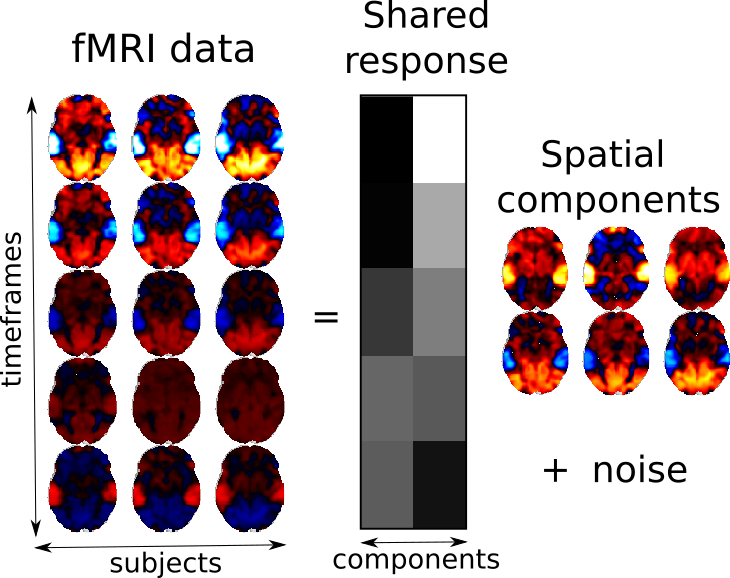
\includegraphics[scale=0.3]{figures/srm/conceptual_figure31.png}
  \caption{\textbf{Shared response model}: The raw fMRI data are modeled as a weighted combination of subject-specific spatial components with additive noise. The weights are shared between subjects and constitute the shared response to the stimuli.}
  \label{fig:srm:conceptual_figure}
\end{figure}

In~\cite{chen2015reduced, anderson2016enabling}, two versions of the shared response model are
introduced which we now present.
\subsubsection{Deterministic shared response model}
\label{sec:deterministicsrm}
The deterministic shared response model sees both $A_i$ and $\sbb$ as parameters to be
estimated and $\forall i, \Sigma_i=\sigma^2 I_v$ where $\sigma$ is an hyper-parameter.
The model is optimized by maximizing the log-likelihood.
The likelihood is given by: $p(\xb) = \prod_i \Ncal(\xb_i; A_i \sbb, \sigma^2 I)$ and
therefore the negative log-likelihood is given up to a constant independent of
$A_i$ and $\sbb$ by:
\begin{align}
  \loss = \sum_i \|A_i \sbb - \xb_i \|^2 = \| \sbb \|^2 -2 \langle A_i \sbb, \xb_i \rangle + \| \xb_i \|^2
  \label{eq:detsrmloss}
\end{align}
The negative log-likelihood $\loss$ is optimized by performing alternate minimization on $(A_1 \dots A_m)$
and $\sbb$. Note that the hyper-parameter $\sigma$ does not have an influence on
the loss and can therefore be safely ignored.

The gradient with respect to $\sbb$ is given by $ \sum_i A_i^{\top}(A_i \sbb -
\xb_i) = \sum_i (\sbb -
A_i^{\top} \xb_i)$
yielding the closed form updates:
\begin{equation}
  \sbb \leftarrow  \frac1m \sum_i (A_i^{\top} \xb_i)
  \label{eq:srm:supdate}
\end{equation}

From \eqref{eq:detsrmloss}, minimizing $\loss$ with respect to $A_i$ is
equivalent to maximize $\langle A_i, \xb_i \sbb^{\top} \rangle$ and therefore we
have:
\begin{equation}
  A_i \leftarrow  \Pcal(\xb_i \sbb^T)
  \label{eq:detsrm:Aiupdate}
\end{equation}
where $\Pcal$ is the projection on the Stiefel manifold: $\Pcal(M) = M
(M^{\top}M)^{-\frac12}$.

The complexity of Deterministic SRM is in $\bigO(\mathrm{n_{iter}} mpvn)$ where
$n$ is the number of samples and $\mathrm{n_{iter}}$ the number of iterations.
We monitor the convergence by looking at the $\ell_{infty}$ norm of the
gradient. We can monitor the gradient without any increase in complexity.
Indeed, after the updates with respect to each mixing matrix have been
carried, only the gradient with respect to $\sbb$ remains: $\sum_i
(\sbb - A_i^{\top}\xb_i)$. The algorithm is stopped when the
gradient is below a chosen tolerance.

\subsubsection{Probabilistic SRM}
\label{sec:probabilisticsrm}
In Probabilistic SRM , $\Sigma_i=\sigma_i^2 I_v$ and the shared
components are assumed to be Gaussian $\sbb \sim \Ncal(0, \Sigma_s)$.
In~\cite{chen2015reduced}, $\Sigma_s$ is only assumed to be definite positive. However,
as will be seen in the FastSRM chapter, enforcing a diagonal $\Sigma_s$ ensures
identifiability (provided the diagonal values are different). So we assume for
now on, that $\Sigma_s$ is diagonal.

The model is optimized via the expectation maximization algorithm.
Denoting $\VV[\sbb | \xb] = (\sum_i \frac1{\sigma_i^2} I +
\Sigma_s^{-1})^{-1}$ and $\EE[\sbb | \xb] = \VV[\sbb | \xb] \sum_i \frac1{\sigma_i^2}
A_i^{\top}\xb_i$, we have
\begin{align}
  p(\xb, \sbb) &= \prod_i \frac{\exp(-\frac{\|\xb_i - A_i \sbb \|^2}{2 \sigma_i^2})}{(2 \pi \sigma_i^{2v})^{\frac12}} \frac{\exp(-\frac12 \langle \sbb , \Sigma_s^{-1} \sbb \rangle )}{(2 \pi | \Sigma_s|)^{\frac12}} \\
               &= c_1 \exp(-\frac12 \left( \sum_i \frac1{\sigma_i^2}\|\xb_i\|^2 - 2  \langle \sum_i \frac1{\sigma_i^2} A_i^{\top}\xb_i, \sbb \rangle \right. \\& \left.+ \sum_i \frac1{\sigma_i^2} \| \sbb \|^2 + \langle \sbb, \Sigma_s^{-1} \sbb \rangle  \right)) \\
               &= c_2 \exp(-\frac12 \left( \langle  \sbb - \EE[\sbb | \xb], \VV[\sbb | \xb]^{-1} ( \sbb - \EE[\sbb | \xb])  \rangle \right)) \label{probsrmcompleted}
\end{align}
where $c_1 = \frac1{(2 \pi \sigma_i^{2v})^{\frac12}}\frac1{(2 \pi |
  \Sigma_s|)^{\frac12}}$ and $c_2 = c_1 \exp(-\frac12( \sum_i
\frac1{\sigma_i^2}\|\xb_i\|^2 - \langle  \EE[\sbb | \xb], \VV[\sbb | \xb]^{-1} \EE[\sbb | \xb] \rangle))$ are independent of $\sbb$.
Therefore $\sbb| \xb \sim \Ncal(\EE[\sbb | \xb], \VV[\sbb, \xb])$

The negative completed log-likelihood is given by
\begin{align}
	\loss = \sum_i \frac12 v \log(\sigma_i^2) + \frac1{2 \sigma_i^2} \| \xb_i - A_i \sbb \|^2
\end{align}
updates are therefore given by:
\begin{align}
&\sigma_i^2 \leftarrow \frac1{v} (\| \xb_i - A_i \EE[\sbb|\xb]\|^2 + \| \diag(\VV[\sbb | \xb]) \|^2) \\
  &A_i \leftarrow \Pcal(\xb_i \EE[\sbb|\xb]^{\top}) \label{eq:psrm:Aiupdate} \\
  & \Sigma_s \leftarrow \VV[\sbb | \xb] + \EE[\sbb | \xb] \EE[\sbb | \xb]^{\top}
\end{align}

It is useful to access the log-likelihood to check the implementation of the
algorithm and monitor the convergence. From equation~\eqref{probsrmcompleted},
the likelihood is given by:
\begin{align}
  p(\xb) &= c_2 \int_{\sbb} \exp(-\frac12 \left( \langle  \sbb - \EE[\sbb | \xb], \VV[\sbb | \xb]^{-1} ( \sbb - \EE[\sbb | \xb])  \rangle \right)) d\sbb \\
         &= c_2 (2 \pi |\VV[\sbb | \xb]|)^{\frac12}
\end{align}
and so up to constants the negative log-likelihood is given by:
\begin{align}
  -\log(p(\xb)) = &\sum_i \frac{v}{2} \log(\sigma_i^2) + \frac12 \log(|\Sigma_s|) - \frac12 \log(|\VV[\sbb | \xb]|) \\ &+ \sum_i
  \frac12 \frac1{\sigma_i^2}\|\xb_i\|^2 - \frac12 \langle  \EE[\sbb | \xb], \VV[\sbb | \xb]^{-1} \EE[\sbb | \xb] \rangle
\end{align}

The complexity of Probabilistic SRM is $\bigO(\mathrm{n_{iter}} mpvn)$, the same as in
Deterministic SRM.
We can monitor the convergence by looking at the log-likelihood decrease at each iteration
and stop the algorithm when the magnitude of the decrease is below some
tolerance.
The storage requirements of Deterministic or Probabilistic SRM are in
$\bigO(mvn)$ which simply means that the dataset needs to hold in memory.

% \section{Related Work}
% \label{sec:rel_work}
% %

% %
% %

% %
% %
% %

% \textbf{Structured mixing matrices} One strength of our model is that we only assume that the mixing matrices are invertible and still enjoy identifiability whereas some other approaches impose additional constraints. For instance tensorial methods~\cite{beckmann2005tensorial} assume that the mixing matrices are the same up to diagonal scaling.
% %
% Other methods impose a common mixing matrix~\cite{cong2013validating, grin2010independent, calhoun2001fmri, Monti18UAI}. Like PCA, the Shared Response Model~\cite{chen2015reduced} (SRM) assumes orthogonality of the mixing matrices. While the model defines a simple likelihood and provides an efficient way to reduce dimension, the SRM model is not identifiable as shown in appendix~\ref{sec:app_identifiability}, and the orthogonal constraint may not be plausible.
% %

% \textbf{Matching components a posteriori} A different path to multi-subject ICA is to extract independent components with individual ICA in each subject and align them. We propose a simple baseline approach to do so called \emph{PermICA}.
% Inspired by the heuristic of the hyperalignment method~\cite{haxby2011common} we choose a reference subject and first match the components of all other subjects to the components of the reference subject. The process is then repeated multiple times, using the average of previously aligned components as a reference. Finally, group components are given by the average of all aligned components. We use the Hungarian algorithm to align pairs of mixing matrices~\cite{tichavsky2004optimal}.
% %
% Alternative approaches involving clustering have also been developed~\cite{esposito2005independent,bigdely2013measure}.

% \textbf{Deep Learning} Deep Learning methods, such as convolutional auto-encoders (CAE), can also be used to find the subject specific unmixing~\cite{chen2016convolutional}. While these nonlinear extensions of the aforementioned methods are interesting, these models are hard to train and interpret. In the experiments on fMRI data in appendix~\ref{appendix_reproduce}, we obtain better accuracy with MultiView ICA than that of CAE reported in~\cite{chen2016convolutional}.

% \textbf{Correlated component analysis} Other methods can be used to recover the shared neural responses such as the correlated component approach of Dmochowski~\cite{dmochowski2012correlated}. We benchmark our method against its probabilistic version~\cite{kamronn2015multiview} called BCorrCA in Figure~\ref{fig:meg}. Our method yields much better results. 

% \textbf{Autocorrelation} Another way to perform ICA is to leverage spectral diversity of the components rather than non-Gaussianity.
% %
% These methods are popular alternative to non-Gaussian ICA in the single-subject setting~\cite{tong1991indeterminacy, belouchrani1997blind, pham1997blind} and they output significantly different components than non-Gaussian ICA~\cite{delorme2012independent}.
% %
% Extensions to multiview problems have been proposed~\cite{lukic2002ica, congedo2010group}.